\documentclass{beamer}


\usepackage[utf8]{inputenc}
\usepackage{amsmath}
\usepackage{amsfonts}
\usepackage{amssymb}
\usepackage{graphicx}
\usepackage{ragged2e}  % `\justifying` text
\usepackage{booktabs}  % Tables
\usepackage{tabularx}
\usepackage{tikz}      % Diagrams
\usetikzlibrary{calc, shapes, backgrounds}
\usepackage{amsmath}
\usepackage{amssymb}
\usepackage{dsfont}
\usepackage{url}       % `\url
\usepackage{listings}  % Code listings
\usepackage[T1]{fontenc}
\usepackage[percent]{overpic}
\usetikzlibrary{trees}
\usepackage[absolute,overlay]{textpos}
\usepackage{tcolorbox}

\newtcolorbox{terminal}{colback=black!70!white,colframe=black!70!white}
\newtcolorbox{focus}{colback=black!10!white,colframe=black!10!white}
\newtcolorbox{terminal2}[1]{colback=white,colframe=black!70!white,fonttitle=\bfseries,title=#1}

\usepackage{theme/beamerthemehbrs}

\author[BAU]{Hassan Umari}
\title{ROS Workshop}
\subtitle{Packages, Tools, and Libraries}
\institute[BAU]{Al-Balqa Applied University}
\date{\today}
\subject{ROS workshop}

% \thirdpartylogo{path/to/your/image}


\begin{document}
{
\begin{frame}
\titlepage
\end{frame}
}



%-------------------------------------------------
\section{Packages}

\begin{frame}{ROS Packages}  
	Inside a ROS package:
	
	\vspace{0.5cm}
	\centering
	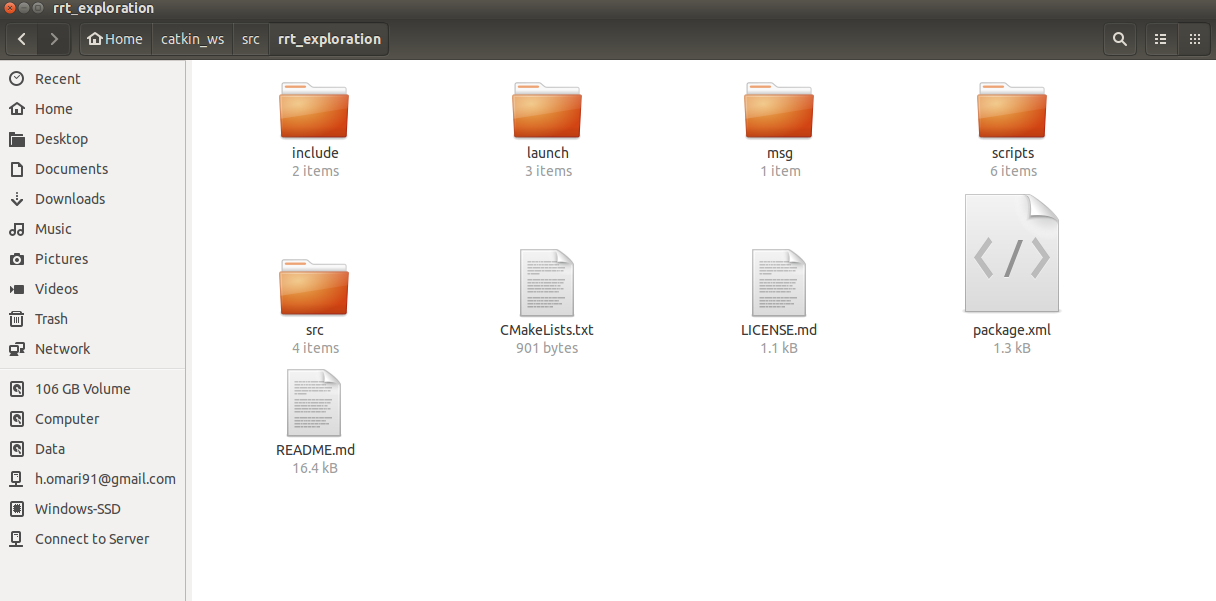
\includegraphics[width=.9\linewidth]{figures/example_package.png}
\end{frame}

\begin{frame}{ROS Packages}    
	\centering
	\scalebox{0.9}{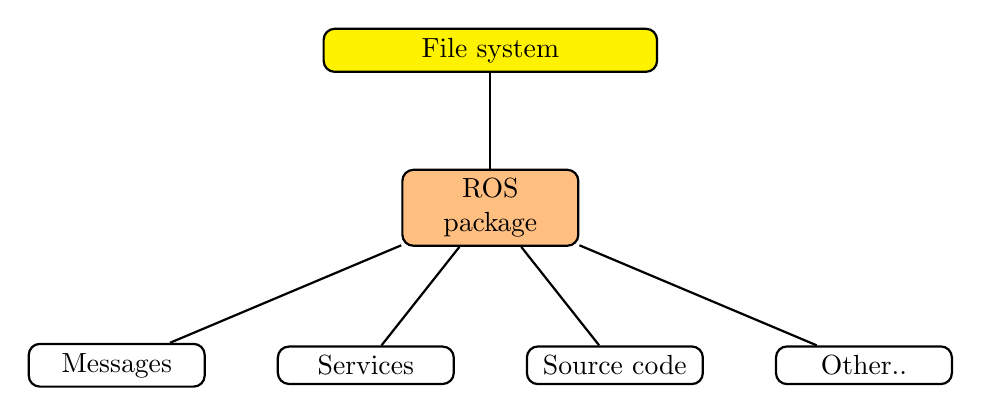
\begin{tikzpicture}[sibling distance=9em, level distance = 2.0cm, thick,
		every node/.style = {shape=rectangle, rounded corners,
			draw, align=center}]]
		\node [text width=4cm, fill = yellow]{File system}
		child { node [text width=2cm, fill = orange!50]{ROS package} 
			child { node [text width=2cm]{Messages} }
			child { node [text width=2cm]{Services} }
			child { node [text width=2cm]{Source code} }
			child { node [text width=2cm]{Other..} }
		};
		\end{tikzpicture}}
\end{frame}

\begin{frame}{ROS Packages}  
	\centering
	\scalebox{0.9}{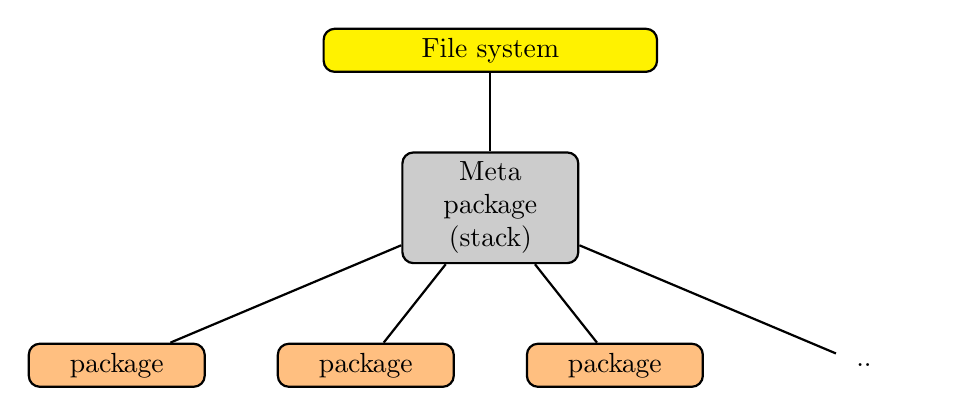
\begin{tikzpicture}[sibling distance=9em, level distance = 2.0cm, thick,
		every node/.style = {shape=rectangle, rounded corners,
			draw, align=center}]]
		\node [text width=4cm, fill = yellow]{File system}
		child { node [text width=2cm, fill = black!20]{Meta package \\ (stack)} 
			child { node [text width=2cm, fill = orange!50]{package} }
			child { node [text width=2cm, fill = orange!50]{package} }
			child { node [text width=2cm, fill = orange!50]{package} }
			child { node [text width=2cm, fill = none, draw = none]{..} }
		};
		\end{tikzpicture}}
\end{frame}

\begin{frame}{ROS Packages}  
	How to install packages:
	\vspace{0.5cm}
    \begin{itemize}
	\item From source (many packages available on GitHub).
		\vspace{0.5cm}
	\item Using \textbf{apt}. Example:
		\vspace{0.5cm}
		 \begin{terminal}
			\color{green} \ttfamily{sudo apt install ros-noetic-navigation}
		\end{terminal}
\end{itemize}  
\end{frame}
%-------------------------------------------------

\setbeamercolor{background canvas}{bg=black}
\begin{frame}[plain]{}  
	\centering
	{\huge \textcolor{white}{Demo} }
	\linebreak
	{\textcolor{white}{package, rosrun, launch files} }
\end{frame}
\setbeamercolor{background canvas}{bg=white}

%-------------------------------------------------
\section{Gazebo}
\begin{frame}{Gazebo}  

	\begin{itemize}
		\item Gazebo is a simulator that is bundled with ROS distributions.
		\vspace{0.5cm}
		\item Gazebo includes a physics engine, 3D rendering (OpenGL), and support for simulating sensors and actuators.
		\vspace{0.5cm}
		\item Simulation environment can be defined in a \ttfamily{.world} file.
	\end{itemize}  
\end{frame}

\setbeamercolor{background canvas}{bg=black}
\begin{frame}[plain]{}  
	\centering
	{\huge \textcolor{white}{Example} }
\end{frame}
\setbeamercolor{background canvas}{bg=white}

%-------------------------------------------------
\section{RViz}
\begin{frame}{RViz}  
	
	\begin{itemize}
		\item RViz can be used to \textbf{visualize} several commonly used ROS messages
		\vspace{0.5cm}
		\item Examples: laser scans, occupancy gird maps, point clouds, images, robot frames, etc..
	\end{itemize}  
\end{frame}

\setbeamercolor{background canvas}{bg=black}
\begin{frame}[plain]{}  
	\centering
	{\huge \textcolor{white}{RViz} }
\end{frame}
\setbeamercolor{background canvas}{bg=white}



%-------------------------------------------------
\section{Coordinate Frames}
\begin{frame}{Coordinate Frames}  
	
	\begin{itemize}
		\item A robotic system involves several coordinate frames that change over time.
		\vspace{0.5cm}
		\item A common task in robotics, is to find the transformation between frames.
		\vspace{0.5cm}
		\item Visualization of these frames is also very important.
	\end{itemize}  
\end{frame}


\begin{frame}{Coordinate Frames} 
	\centering
	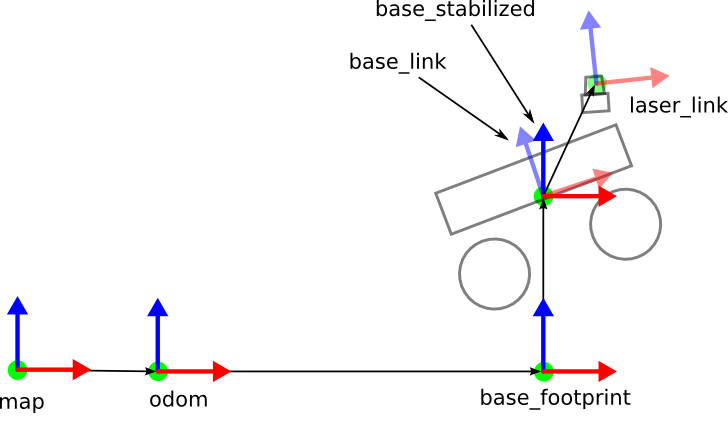
\includegraphics[width=.8\linewidth]{figures/coordsystems_img.png} 
	\begin{textblock}{10}(1,14)
		\tiny{image source: http://wiki.ros.org/hector\_slam/Tutorials/SettingUpForYourRobot}
	\end{textblock} 	
\end{frame}

\begin{frame}{Coordinate Frames} 
	\centering
	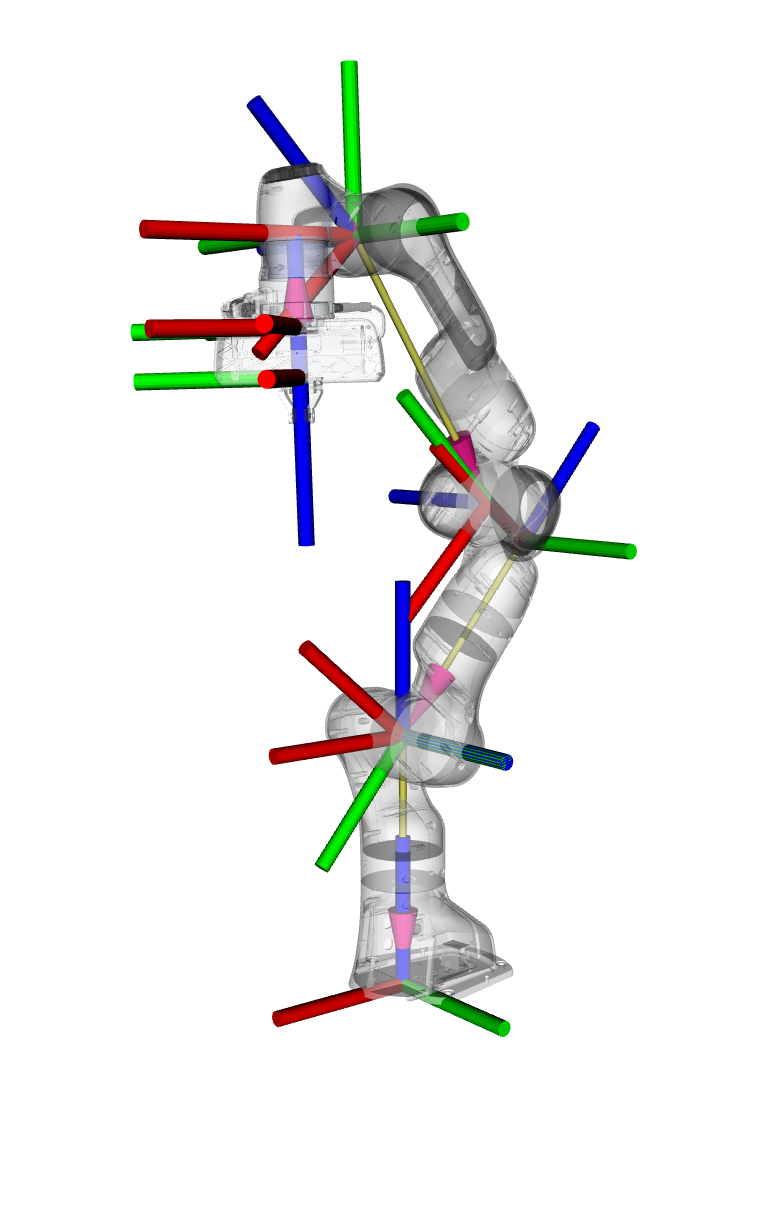
\includegraphics[width=.4\linewidth]{figures/panda_tf.png} 
	\scalebox{.5}{Source: https://ros-planning.github.io/moveit\_tutorials/doc/robot\_model\_and\_robot\_state/robot\_model\_and\_robot\_state\_tutorial.html}	
\end{frame}

\subsection{tf - The Transform Library}
\begin{frame}{tf - The Transform Library} 
	\subtitle{Coordinate Frames}
	\begin{itemize}
	\item The tf is a library for handling \textbf{transformation} between frames. 
	\vspace{0.5cm}
	\item The library stores the relationship between frames in a \textbf{tree} structure buffered in \textbf{time}.
	\vspace{0.5cm}
	\item In ROS, it comes as a package called \textbf{tf2}.
\end{itemize}
\end{frame}

\begin{frame}{tf - The Transform Library} 
	\subtitle{Coordinate Frames}
	\centering
	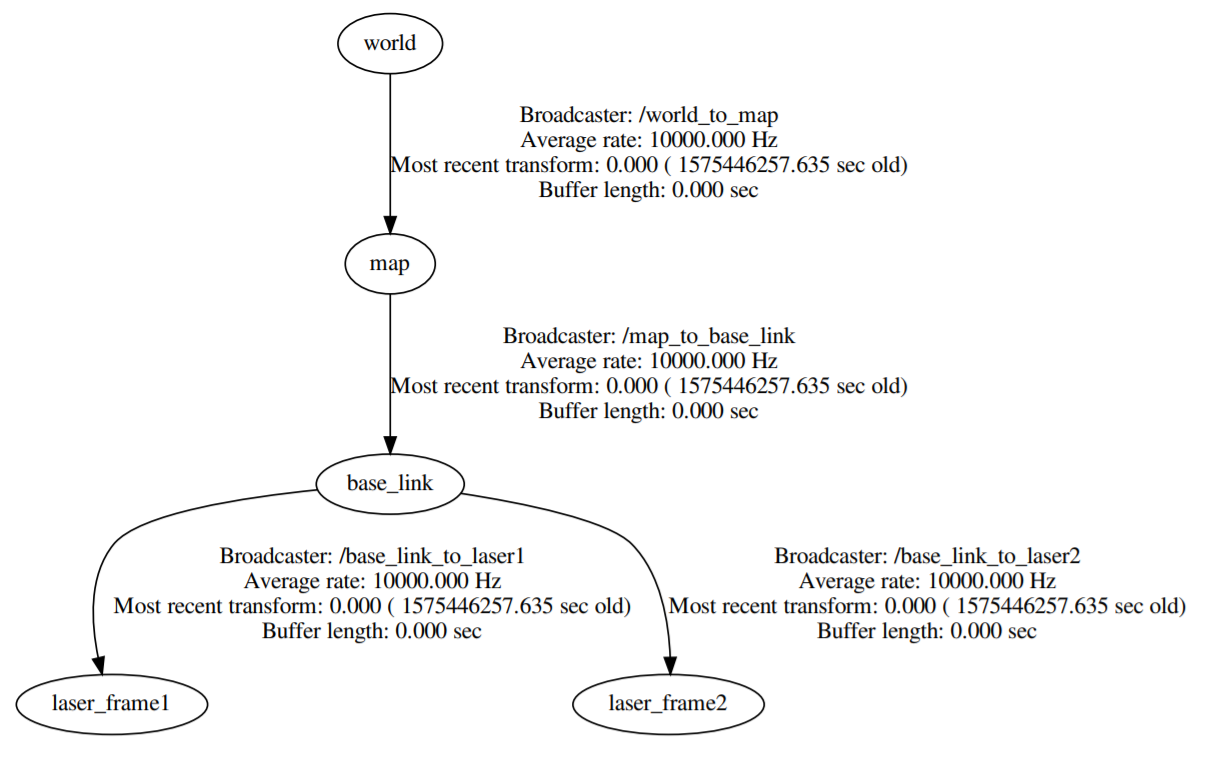
\includegraphics[width=.9\linewidth]{figures/tf_tree.png} 
	\scalebox{.5}{Source: https://spl.hevs.io/spl-docs/tools/ros/tf2.html}	
\end{frame}


\begin{frame}{tf - The Transform Library} 
	\subtitle{Coordinate Frames}

	\begin{itemize}
		\item There is no central server. Each client listens to published transforms and maintains a copy of the tree.
		\vspace{0.5cm}
		\item What a node can do:
		\begin{itemize}
			\item Broadcast a transformation
			\item Listens for all transformations
			\item query for a transform at a chosen time instance
		\end{itemize} 
		\vspace{0.5cm}
		\item Comes with a tool to quickly publish static transformations.
	\end{itemize}
\end{frame}

\setbeamercolor{background canvas}{bg=black}
\begin{frame}[plain]{}  
	\centering
	{\huge \textcolor{white}{Demo} }
\end{frame}
\setbeamercolor{background canvas}{bg=white}


\begin{frame}{URDF} 
	\begin{itemize}
		\item URDF = Unified Robotics Description Format
		\vspace{0.5cm}
		\item XML format for representing a robot model
	\end{itemize}
\end{frame}


\begin{frame}[fragile]{URDF}
	\lstset{language=xml,
		basicstyle=\scriptsize,
		keywordstyle=\color{blue}\ttfamily,
		stringstyle=\color{red}\ttfamily,
		commentstyle=\color{green}\ttfamily,
		morecomment=[l][\color{magenta}]{\#},
		showstringspaces=false
	}
	\begin{lstlisting}
	<robot>
		<link>
		...
		</link>
		<link>
		...
		</link>
		
		<joint>
		...
		</joint>
		
	</robot>
	\end{lstlisting}
\end{frame}

\begin{frame}{URDF} 
	\begin{itemize}
		\item URDF file can be loaded by \textbf{robot\_state\_publisher}
		\vspace{0.5cm}
		\item It will publish link frames to tf
	\end{itemize}
\end{frame}

\setbeamercolor{background canvas}{bg=black}
\begin{frame}[plain]{}  
	\centering
	{\huge \textcolor{white}{Example} }
	\linebreak
	{\textcolor{white}{URDF + Robot state publisher} }
\end{frame}
\setbeamercolor{background canvas}{bg=white}


%-------------------------------------------------
\section{Popular Packages}
\subsection{Gmapping}
\begin{frame}{Gmapping} 
	\begin{itemize}
		\item Is a ROS wrapper for Gmapping C++ library.
		\vspace{0.5cm}
		\item Implements a SLAM algorithm.
		\vspace{0.5cm}
		\item odometry + laser scan $\rightarrow$ occupancy grid map 
	\end{itemize}
\end{frame}

\begin{frame}{Occupancy Grids} 
	\subtitle{Gmapping}
	\centering
	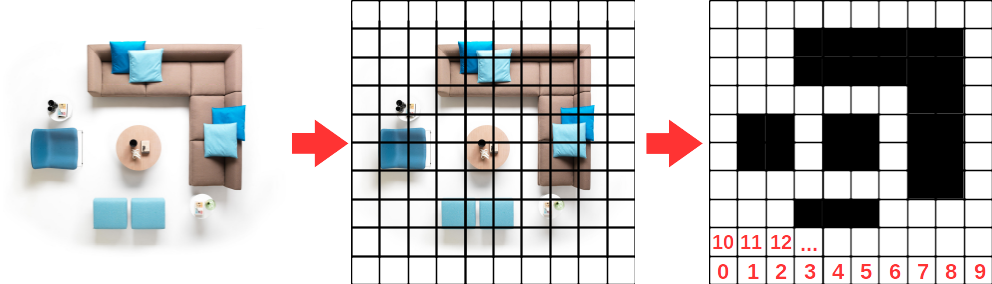
\includegraphics[width=.99\linewidth]{figures/occupancy_grid.png} 
	\vspace{0.5cm}
	\begin{focus}
		\scalebox{.8}{\ttfamily{map data = [0, 0, 0, 0, ... , 0, 100 ,100 ,100 ,0 ,0 , ... ]}}
	\end{focus}
\end{frame}

\begin{frame}{Occupancy Grids} 
	\subtitle{Gmapping}
	\centering
	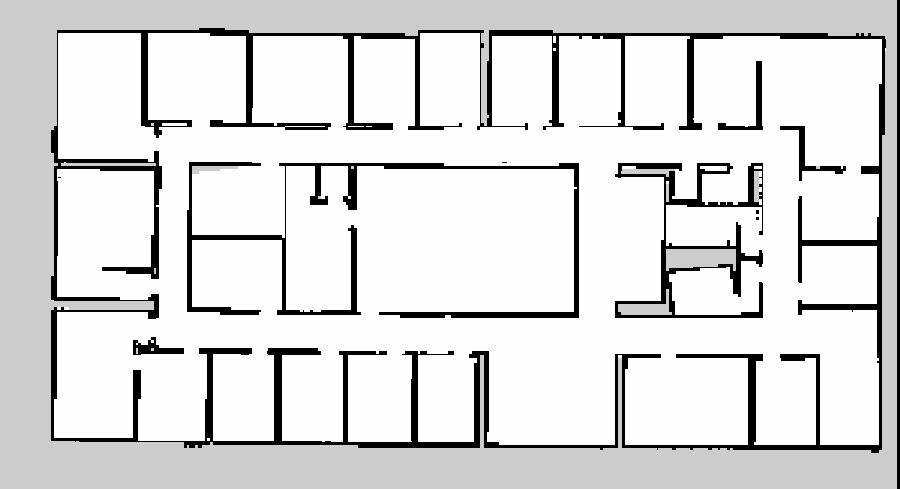
\includegraphics[width=.99\linewidth]{figures/map.png} 
\end{frame}

\begin{frame}{Gmapping}
		\begin{terminal}
			\color{green} \ttfamily{sudo apt install ros-noetic-gmapping}
		\end{terminal}
\end{frame}

\setbeamercolor{background canvas}{bg=black}
\begin{frame}[plain]{}  
	\centering
	{\huge \textcolor{white}{Gmapping} }
\end{frame}
\setbeamercolor{background canvas}{bg=white}


\subsection{Navigation Stack}

\begin{frame}{Navigation Stack} 
	\begin{itemize}
		\item A collection of packages for mobile robot \textbf{navigation} (\textbf{2D})
		\vspace{0.5cm}
		\item map + odometry + laser scan + goal $\rightarrow$ velocity commands
	\end{itemize}
\end{frame}


\begin{frame}{Navigation Stack} 
	\begin{itemize}
	\item Costmap
	\vspace{0.5cm}
	\item Global planner
	\vspace{0.5cm}
	\item Local planner	
\vspace{0.5cm}	
\end{itemize}
\end{frame}

\begin{frame}{Costmap} 
	\subtitle{Navigation Stack}
	\centering
	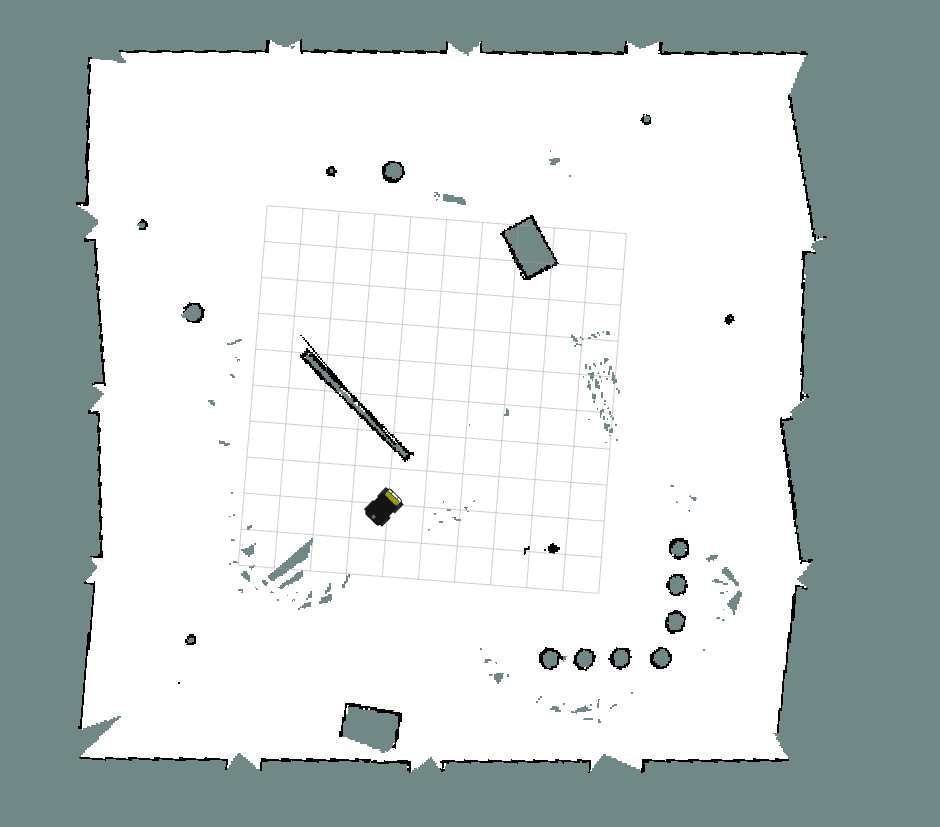
\includegraphics[width=.7\linewidth]{figures/costmap_0.png}
\end{frame}

\begin{frame}{Costmap} 
	\subtitle{Navigation Stack}
	\centering
	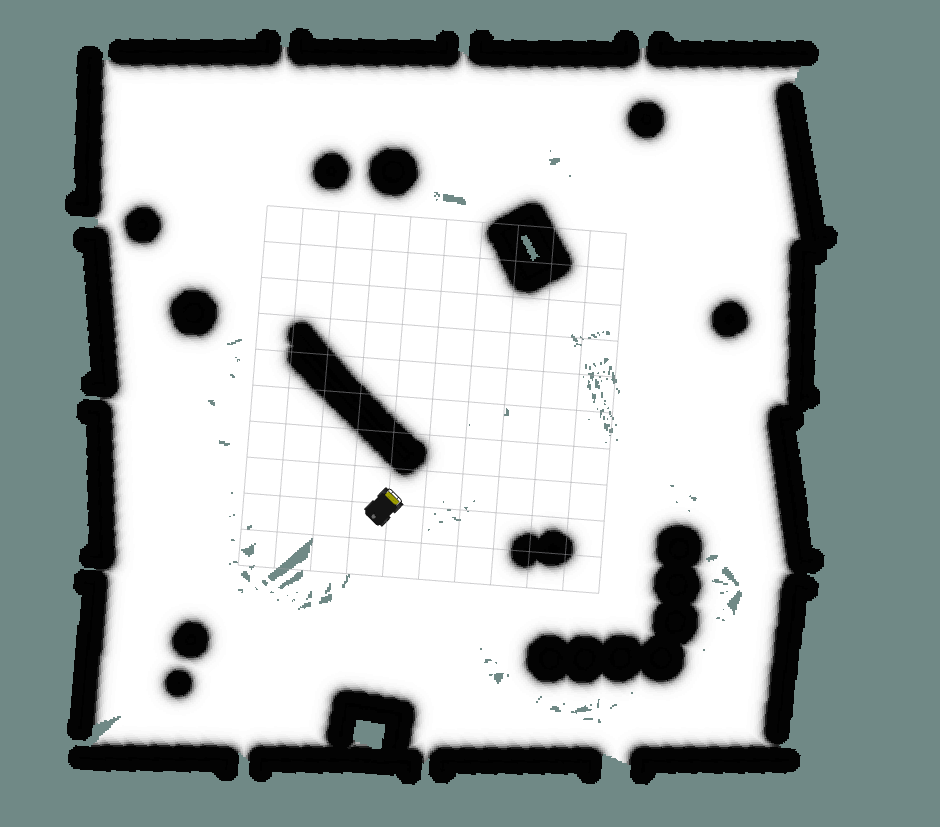
\includegraphics[width=.7\linewidth]{figures/costmap_1.png}
\end{frame}

\begin{frame}{Costmap} 
	\subtitle{Navigation Stack}
	\centering
	
\includegraphics[width=.7\linewidth]{figures/costmap_3.png}
\end{frame}

\begin{frame}{Costmap} 
	\subtitle{Navigation Stack}
	\centering
	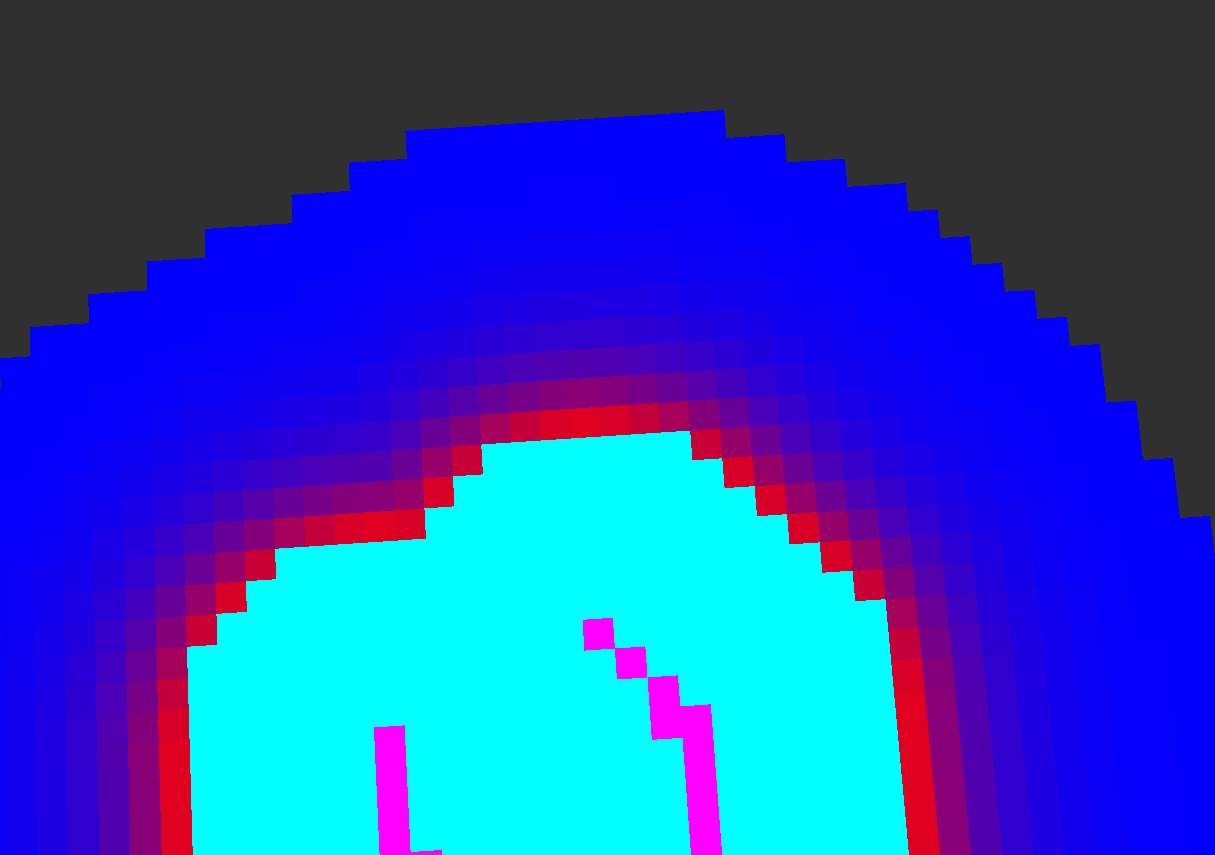
\includegraphics[width=.7\linewidth]{figures/costmap_4.png}
\end{frame}

\begin{frame}{Costmap} 
	\subtitle{Navigation Stack}
	\centering
	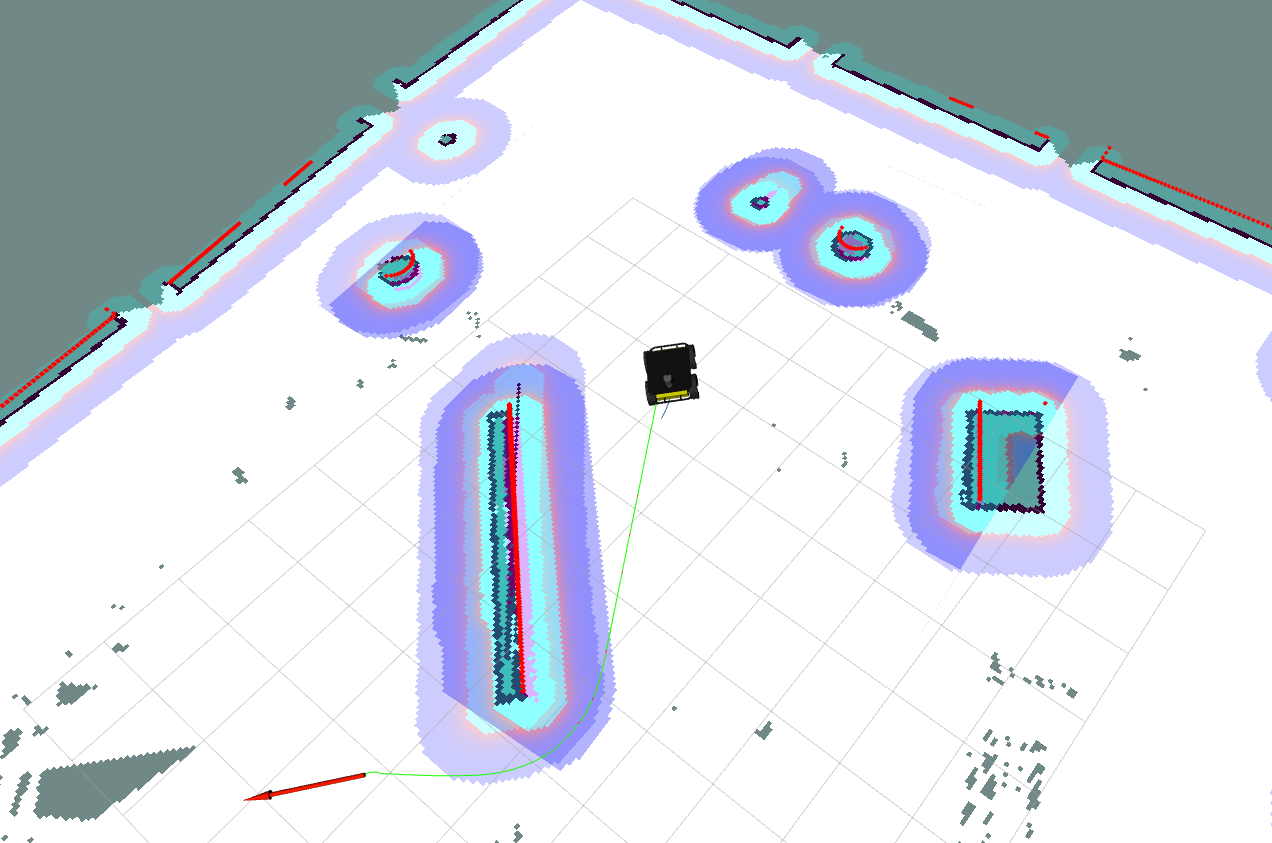
\includegraphics[width=.99\linewidth]{figures/costmap_5.png}
\end{frame}

\begin{frame}{Global Planner}
	\subtitle{Navigation Stack} 
	\begin{itemize}
		\item Uses the \textbf{global costmap}
		\vspace{0.5cm}
		\item \textbf{Search} algorithm to find a safe path in the global costmap
		\vspace{0.5cm}	
	\end{itemize}
\end{frame}

\begin{frame}{Global Planner}
	\subtitle{Navigation Stack} 
	\centering
	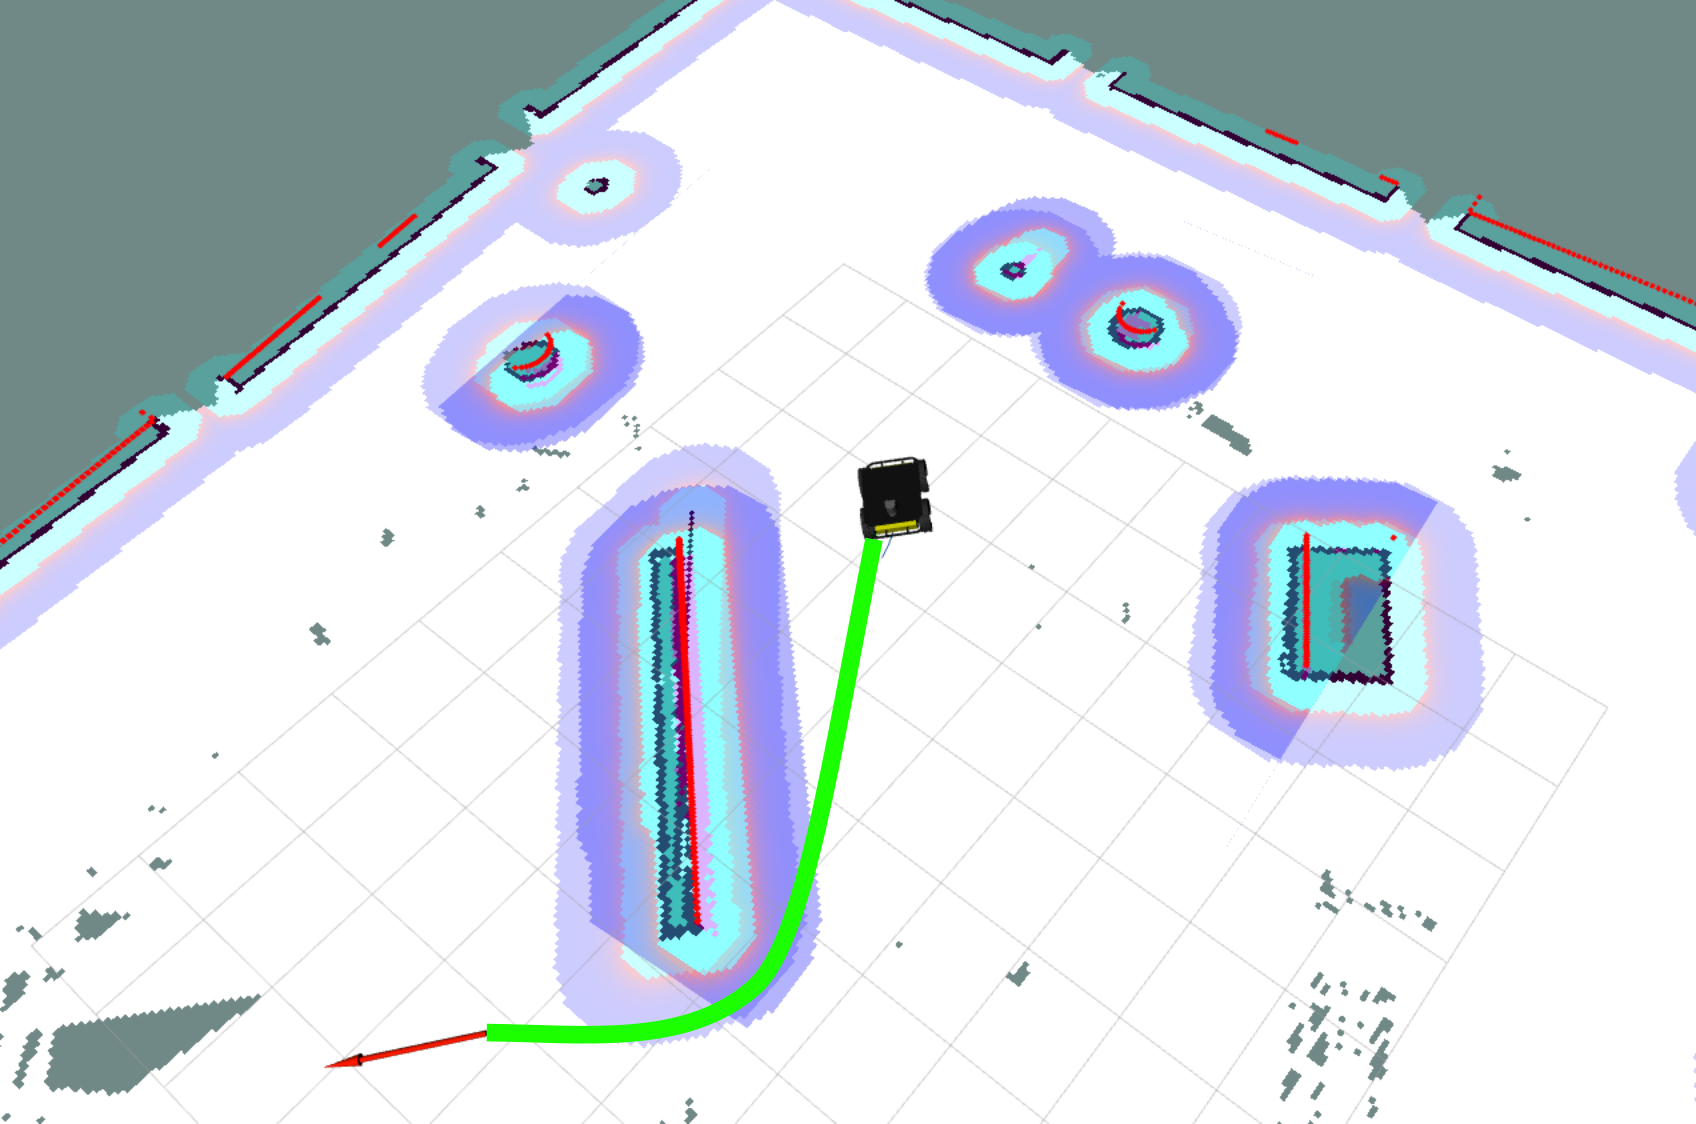
\includegraphics[width=.99\linewidth]{figures/costmap_6.png}
\end{frame}

\begin{frame}{Local Planner}
	\subtitle{Navigation Stack} 
	\begin{itemize}
	\item Generates \textbf{velocity commands} to make the robot \textbf{follow} the global plan
	\vspace{0.5cm}
	\item It uses a \textbf{local costmap}
	\vspace{0.5cm}
	\item A local path is generated based on the global plan
	\vspace{0.5cm}		
\end{itemize}
\end{frame}

\begin{frame}{Local Planner}
	\subtitle{Navigation Stack} 
	\centering
	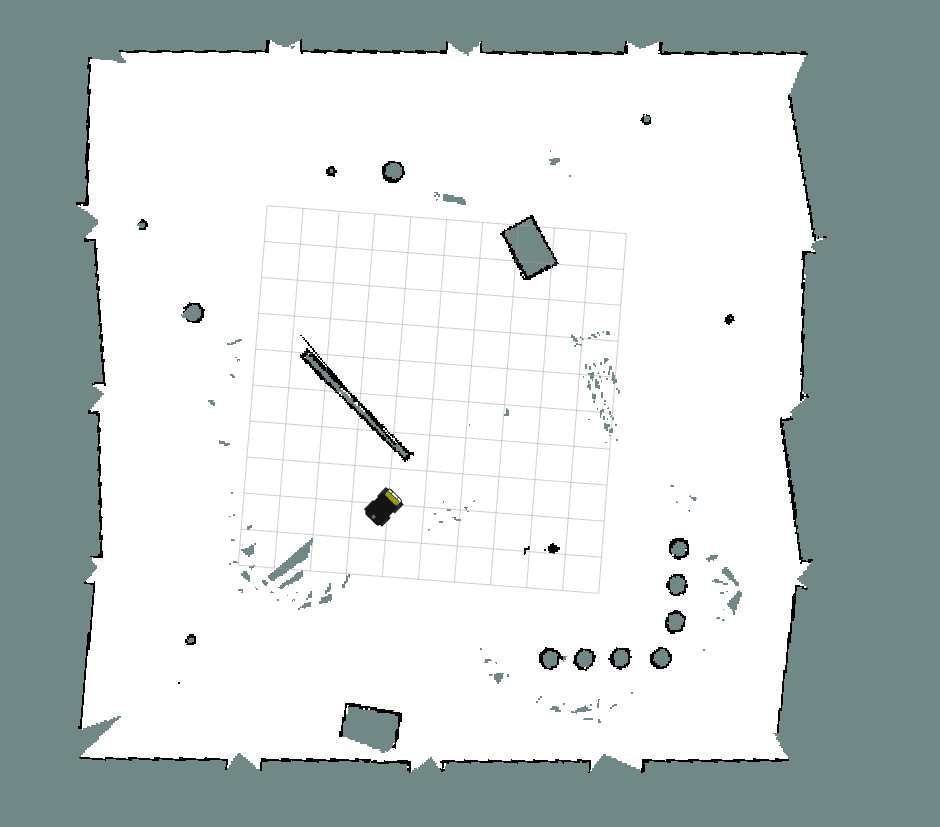
\includegraphics[width=.7\linewidth]{figures/costmap_0.png}
\end{frame}

\begin{frame}{Local Planner}
	\subtitle{Navigation Stack} 
	\centering
	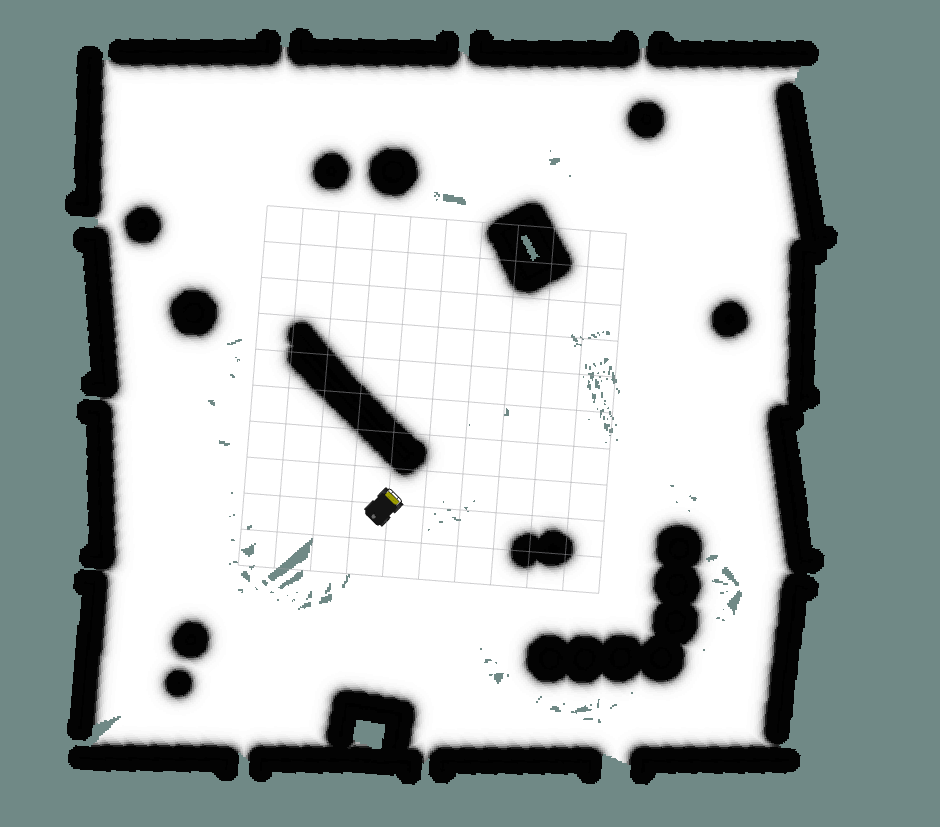
\includegraphics[width=.7\linewidth]{figures/costmap_1.png}
\end{frame}
\begin{frame}{Local Planner}
	\subtitle{Navigation Stack} 
	\centering
	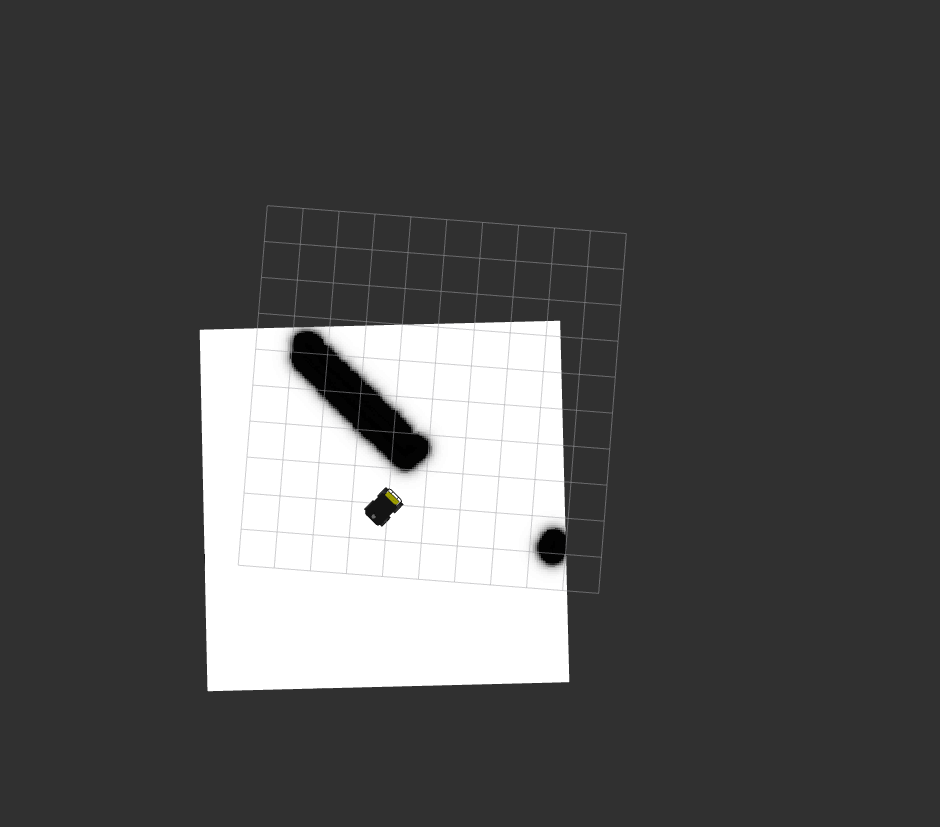
\includegraphics[width=.7\linewidth]{figures/costmap_2.png}
\end{frame}

\setbeamercolor{background canvas}{bg=black}
\begin{frame}[plain]{}  
	\centering
	{\huge \textcolor{white}{Demo} }
\end{frame}
\setbeamercolor{background canvas}{bg=white}


\setbeamercolor{background canvas}{bg=black}
\begin{frame}[plain]{}  
	\centering
	{\huge \textcolor{white}{Thank you} }
	\linebreak
	\vspace{1.0cm}
	{\huge \textcolor{white}{Questions..?} }
\end{frame}
\setbeamercolor{background canvas}{bg=white}

\end{document}
% references:
% http://wiki.ros.org/tf2
% https://www.mathworks.com/help/sm/ug/urdf-model-import.html
% http://wiki.ros.org/urdf
% http://wiki.ros.org/gmapping
% https://openslam-org.github.io/

% api
% http://docs.ros.org/en/melodic/api/tf/html/python/